\documentclass[conference]{IEEEtran}
\usepackage{cite}
\usepackage{amsmath,amssymb,amsfonts}
\usepackage{algorithmic}
\usepackage{graphicx}
\usepackage{subcaption}
\usepackage{textcomp}
\usepackage{xcolor}
\def\BibTeX{{\rm B\kern-.05em{\sc i\kern-.025em b}\kern-.08em
    T\kern-.1667em\lower.7ex\hbox{E}\kern-.125emX}}
\begin{document}

\title{sHeap: Mitigating Dangling Pointers\\}

\author{\IEEEauthorblockN{Matt McCreesh}
\IEEEauthorblockA{\textit{Stevens Institute of Technology}\\
mmccrees@stevens.edu}
\and
\IEEEauthorblockN{Thomas Pyle}
\IEEEauthorblockA{\textit{Stevens Institute of Technology}\\
tpyle@stevens.edu}
\and
\IEEEauthorblockN{Connor Zapfel}
\IEEEauthorblockA{\textit{Stevens Institute of Technology}\\
czapfel@stevens.edu}
}

\maketitle

\begin{abstract}
When an object in memory is deallocated, the freed memory can still be accessible 
by the program if any pointers to it are not nullified. Pointers left pointing 
to objects that have been freed are referred to as dangling pointers. They 
point to a location that once had a valid object of the type they point to but 
no longer does. The presence of such pointers can lead to use-after-free 
vulnerabilities. These vulnerabilities can be just as worrisome as spatial 
memory errors like buffer overflows, as they can be used by an attacker to 
hijack the control flow of an application. In this paper, we propose and evaluate 
a runtime allocator, sHeap, which mitigates the dangers of use-after-free 
vulnerabilities by preventing arbitrary code execution through dangling 
pointers. Our solution is based off ideas and approaches proposed and 
implemented by Cling in \cite{b1}.
\end{abstract}

\begin{IEEEkeywords}
Memory allocator, use-after-free, heap, memory safety
\end{IEEEkeywords}

\section{Introduction}
Dangling pointers to the heap, pointers left pointing to deallocated objects, 
are a major security concern. They were once thought to be too difficult for 
attackers to exploit, as attackers would need to be able to force a program 
to put his data in the same location as the dangling pointer pointed to. 
Because of this, in the past vulnerabilities were sometimes left unpatched 
for long periods of time and written off as non-critical. But as spatial 
memory protections became more popular, the arms race between attackers and 
defenders continued and it was shown that attackers could reliably exploit 
use-after-free vulnerabilities. Heap Spraying and Heap Feng Shui allows an 
attacker to reliably align his own data with that of a dangling pointer. 
This means that reliable exploitation of these vulnerabilities is possible. 
In fact, these vulnerabilities have been showing up in the wild, including 
in a zero-day exploits on the Google Chrome web browser, where a 
vulnerability was patched in March 2019. Use-after-free vulnerabilities are 
very attractive for attackers to exploit because there is potential for 
control flow hijacking. If a dangling pointer to a heap object with 
function pointers exists, an attacker may be able to launch code-reuse 
attacks, such as return-to-libc, by convincing the program to make a 
function call through a dangling pointer.  

An interesting target of attacks is C++ objects.  The C++ language is object based and 
allows for inheritance. In C++, a parent class can declare some functions 
as virtual functions, which can be redefined in derived classes. Virtual 
functions should execute the version of the function of the object that 
is allocated, as opposed to the type of variable pointing to it. In order 
to do this so called virtual function dispatch, C++ objects with virtual 
functions start with a pointer (called the vptr) to a virtual table 
(vtable), which stores function pointers for virtual functions of this 
object. When a virtual function of a C++ object is called, the vptr is 
used to find the vtable, which is used to find the function pointer of 
the correct function. Use-after-vulnerabilities can exploit this virtual 
function dispatch mechanism. If an attacker controls the buffer in the 
heap that overlaps with memory that once contained a C++ object, and 
there is a dangling pointer to that object, the attacker can overwrite 
what was the vptr field was and set it to point to his own counterfeit 
vtable. Then, when the dangling pointer tries to execute a virtual 
function, it will instead execute whatever the attacker points his vtable 
to. 

Unfortunately, use-after-free vulnerabilities have proven very difficult 
to defend against. They are hard to detect with static analysis and code 
reviews, as they require understanding the state of memory when analyzing 
pointer dereferences. Such memory state depends on code that has already 
executed, and synchronization of code execution, making this task 
especially difficult in large applications. To address this problem, we 
introduce and implemented a memory allocator, sHeap. Memory allocator 
changes have been made to address other security issues such as double 
frees and overwrites of heap metadata, so there is precedent in 
implementing security hardening in the run time allocator itself. Our 
solution is based off of ideas proposed in \cite{b1}. sHeap takes many 
elements from Cling, though it does not implement every optimization of 
Cling, as some of the specific optimizations for small allocations are 
left for future work. 

sHeap redefines the memory allocator interfaces (malloc(), new(), 
calloc(), and realloc()) to allow for pooling of allocations over time 
with objects of the same type. sHeap uses the call site to malloc, 
calloc, and realloc to determine the type, assuming that a call site to 
malloc or new will always request memory of the same type. It also does 
malloc wrapper detection to find call sites to simple malloc wrappers so 
as to avoid pooling objects that are of different types because they are 
allocated from wrappers of malloc. Simple malloc wrappers may just check the value returned by malloc or collect statistics before returning what malloc returns. They obscure the real allocation site, sHeap uses to determine allocation type, so they must be unwrapped.  This wrapper detection allows us to find the call site to the new C++ operator, which allows us to properly pool C++ objects and dynamically allocated arrays. 

Our allocator defends against arbitrary code execution through a dangling 
pointer.  It does not prevent dangling pointers from being used, but it 
does ensure that they always point to objects of the same type. Therefore, 
if an attacker tries to execute a function call through a dangling 
pointer, the code executed should be a valid function for an object of 
that type.  sHeap is not concerned with data only attacks where fields 
are overwritten. 

Ultimately, our solution is effective from a security perspective, but it 
has high CPU and memory overhead for some of the benchmarks we used. This 
is likely a result of the fact that sHeap is not currently optimized for 
small allocations.  We focused on supporting allocations of any size to 
make it work for as many programs as possible, so we tailored our project 
to support large allocations instead of also being optimized for small 
allocations.  The use of buckets for small allocations should allow for 
great performance benefits for applications making many small allocations. 
This will result in less system calls and also significantly reduce 
fragmentation. We leave such performance improvements for future work.

\section{Background}

\subsection{Current Heap Implementations}
The most common heap implementation currently in use is GNU malloc, also 
known as dlmalloc. GNU malloc works by allocating blocks of data using mmap 
calls, as well as brk calls, in order to find unavailable blocks to give to 
the use. Malloc does this through the use of a free list which keeps track 
of the size of program-owned memory that is no longer attached to allocated 
blocks.  Most heap implementations, including GNU malloc, do not make any effort to mitigate use-after-free vulnerabilities. 

\subsection{Related Work}
A naive approach to defend against dangling pointers is by preventing any 
heap allocated objects from ever sharing the same memory space. This is done 
by never reusing freed memory, effectively replacing free() with a function 
which does nothing. This clearly will have high physical memory overhead for long running applications. More intelligent implementations of the naive solution aim to signal the operating system to release physical pages while not reusing virtual addresses, but this still can still have high physical memory overhead because of fragmentation, where small allocations hold back pages from being released.  The naive solution is simple implement, but incurs an extremely large overhead of consumed virtual memory.

Some other defenses include probabilistic defenses, such as DieHard \cite{b2}
and Archipelago \cite{b3}. These defenses both rely on defeating 
use-after-free attacks by making it improbable that the attacker will be able 
to align heap objects. It does this by randomly locating objects in a larger 
heap than usual. This of course results in worse memory consumption, because 
the heap needs to be larger in order to ensure the probabilistic defense.

Cling \cite{b1} is a memory allocator which attempts to provide protection 
from dangling pointer in particular through the use of type safety in heap 
allocations. It does this by analyzing the return site of malloc (by looking 
at malloc'’s stack frame), as well as categorizing objects based off this size. 
It does this in order to determine run-time type information based off 
assumptions about the way that programmers frequently perform allocations of data. Cling performs many optimizations and as such is capable of 
reducing runtime and memory overhead to something comparable (and even 
sometimes better) than traditional GNU malloc. 

\section{Design}

\subsection{Objective}
sHeap is designed to protect heap memory in a manner similar to Cling, but 
unfortunately imposes a number of limitations due to the time and resource 
constraints of the team. This means that although Cling is capable of 
optimizing small allocations by storing many in a single allocated block 
\cite{b1}, we were unable to perform this optimization in order to 
prioritize goals such as the detection of wrappers and thread safety.

The implementation of this technique was done by replacing the 4 malloc 
calls defined in traditional glibc. These can all be performed by loading 
our shared library before loading stdlib. This is done by using the 
environment variable LD\_PRELOAD. By redefining these 4 methods, we ensure 
that any programs which use our heap allocator will always have a 
consistent view of the heap through our allocator.

\subsection{Architecture}

\begin{figure}[htbp]
  \centering
  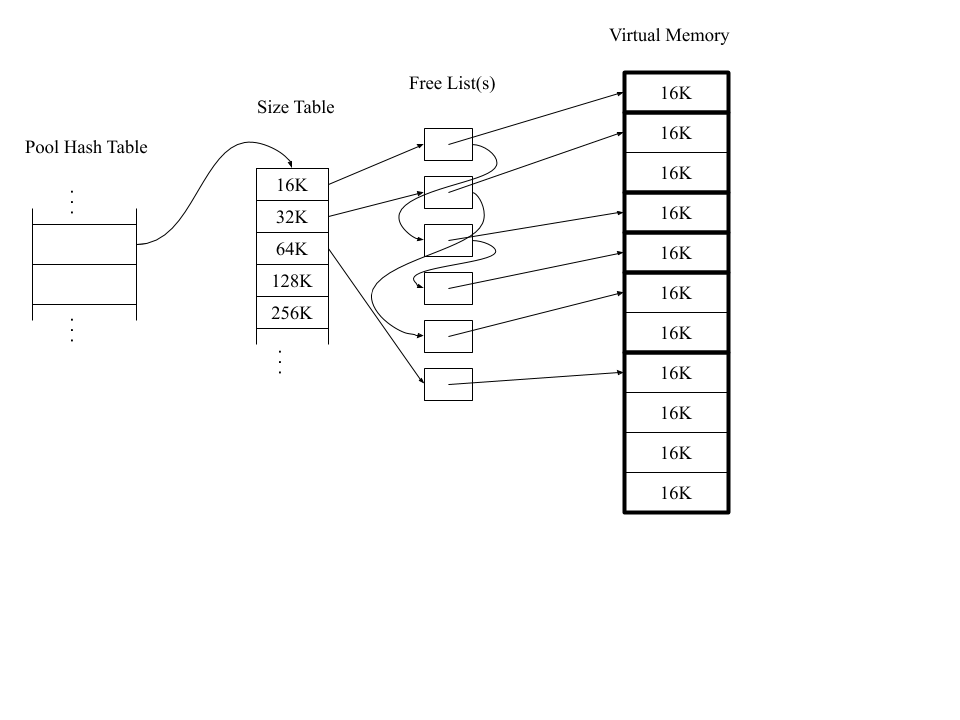
\includegraphics[width=\linewidth]{sheap_model.png}
  \caption{sHeap Architecture Summary.}
  \label{fig:sheap-model}
\end{figure}

sHeap is primarily made up of three coordinating components. First, the 
pool hash table tracks the mapping from allocation sites to their 
corresponding site pools. Then the site pool manages the different pointers 
to the free space available for each size class. The free space is stored 
in a linked list structure called a free list. \ref{fig:sheap-model} 
provides a visual representation of the sHeap architecture. In the next 
three subsections, we will go into the design and purpose of the three 
main components mentioned above.

\subsubsection{Pool Hash Table}
The first layer of interaction into the sHeap ecosystem is the pool hash table 
(PHT). It has a single purpose: to map allocation sites to their appropriate 
site pool. A hash table allows for constant time average case access complexity 
which is essential for maintaining low overhead. The PHT makes use of the 
allocation site in the hash function making for an efficient and 
collision-resistant hash function. The team opted for linear probing as the 
collision handling strategy for simplicity of implementation, and it has proven 
effective in practice. Each entry in the hash table at a minimum needs to store 
a pointer to the isolated allocation site pool in order to connect the 
allocation site to the next stage in the pipeline.

\subsubsection{Site Pool}
The next primary data structure in sHeap is the site pool, also referred to as the size table. This is a struct for 
every allocation site, managing the metadata for each allocation site pool. The 
primary job of this data structure is to manage the pooling of allocations by 
size class, which is why it is referred to as the size table. A size class is a power of 2 KB allocation size starting at 16KB. 
That is, every allocation size of 16KB or less will be in the 0th size class 
and be allocated only 1 block. Any allocation size of 16KB to 32KB will be in 
the first size class and be given 2 blocks. The next size class corresponds 
to an allocation of 4 blocks and is for allocation sizes between 32KB and 64KB. 
The size table structure stores a table of pointers to free lists heads for each 
size class, as well as metadata about allocation sizes used to determine if a 
call site is a wrapper. Every time a new allocation site is found, a site pool 
element is created for that allocation site. For future allocation requests, this 
structure will be used to find the free list head for the size class being 
requested so type safe address space reuse can be done. During future deallocations, 
this table is used to append freed block nodes to the correct free list for the 
allocation site and size class of the original allocation. We will get more into 
the specifics of this when discussing the free lists themselves. The site pool 
structure is also very useful for wrapper detection. By having a field that 
stores the original size requested, as well as whether or not this allocation site 
was determined to be a wrapper or a non-wrapper, we can correctly and efficiently 
find the real allocation site of malloc wrappers, and know when to suspect an 
existing allocation site is a wrapper. We will discuss the importance of this in 
the next section.

\subsubsection{Freelists}
The free list is designed to keep track of previously allocated, but freed, blocks. 
In order to preserve the mitigation described, it is necessary for the free list 
to be dependent on the allocation site and the size class of allocations, and as 
such each pair of allocation and size class has its own free list. The head of 
the free list is stored in the size table, and allocation attempts to find a 
previously allocated node before it attempts to request more allocated memory. The 
free list is designed to make reverse lookups - programmed owned data to free list 
nodes - performed in constant time. This is so that the free operation is performed 
in constant time, and is capable of performing a lookup for the relevant size class 
and type information stored in the node. This is necessary in order to append the 
newly freed node to the correct free list.

\section{Implementation}

\subsection{Pool Hash Table}
As discussed in section 3, the pool hash table exists to store the mapping of 
allocation sites to their site pools. This requires the implementation of a hash 
table that is stored in the out-of-band metaheap. We implemented the hash table as 
a single contiguous array of pht\_entry structs. Each of these structures stores 
exactly two pieces of information: the allocation site and the pointer to the 
corresponding site pool. We have to store the allocation site in the pht\_entry in 
order to detect collisions. If two allocation sites end up hashing to the same 
hash index, there is no way to confirm correctness unless we store that allocation 
site. Our PHT was not dynamically scalable which means the size of the PHT is 
decided at initialization by a constant and doesn’t change throughout the runtime 
of sHeap. This is something that could be improved in the future in order to 
accomodate more allocation sites, but in our testing, this was not an issue that 
we encountered. The hashing algorithm that was used is pretty simple. Since the 
input is an eight-byte pointer (the allocation site), we just isolate xor the 
upper and lower four bytes then mod the result by the size of the PHT as 
dictated by that constant variable from earlier.

\subsection{Site Pool}
Once the PHT has found the site pool for this allocation, which stores the pool metadata for this allocation site, we can discuss how allocation works. 
On the first request from an allocation site, the allocation site will be 
inserted into the PHT but the size table pointer for the pool metadata will be 
null. This will trigger the size table to create a new element for the 
allocation site and update the PHT element to have a pointer to that struct. In 
future allocations from this allocation site, the size table will try to utilize 
the free list for the given size class by passing in the location that it stores 
the free list head pointer to the allocation function. That function, which is discussed further in the next section, will use the freelist for allocations if it is not empty.  The important point is the site pool size table allows sHeap to efficiently find the beginning of the correct free list so blocks can be reused if the free list is not empty. 

\subsection{Freelists}
The free list is implemented as a structure containing all of the relevant type 
information of a block of memory, as well as pointers to the next and previous nodes in the free list. 
The actual allocation operation is passed through the pool hash table and the size 
table, and then arrives at the free list in order to determine whether or not to 
create a new allocated block, or whether to reuse a previously freed block. This 
is done by checking whether the flist passed by the size table contains a valid 
pointer (in which case there is a block to use), and if not, it will push the 
program break and claim a new one. When performing the free operation, sHeap needs 
to lookup the relevant information for the node (its allocation site and its size 
class) in order to find the correct free list to use. It does this by preserving 
the order of the program data with the free list nodes, so the offset of the 
program data from its start (in blocks) corresponds to the free list node to use. 
This allows constant-time reverse lookups of the free list nodes. Once we perform 
the reverse lookup, we are able to use the information stored in the node to 
append it to the appropriate free list, by looking up the allocation site in the 
pool hash table, and then the corresponding size in the size table. The node is 
then appended to the front of that free list, to be reused in a subsequent malloc 
call.

\subsection{Wrapper Detection}
At this point we have shown how our memory allocator works. The security benefits 
we achieve all stem from constraining memory reuse to be within pools of the same type, and aligning those allocations to start at the same positions. Unfortunately, 
using the call site to malloc as the allocation site is not always sufficient for 
uniquely identifying the type of the allocation. Simple malloc wrappers can exist 
in programs and this would subvert our protections. A malloc wrapper is a 
function that calls malloc on behalf of a caller, simply returning the pointer it 
mallocs. We found that the new C++ operator was a malloc wrapper that we needed to be able to handle for type safe memory reuse for C++ programs.  Other common uses of malloc wrappers include checking if the return is null 
before sending it to the caller and collecting statistics on allocations. In order to accurately pool allocations by type, we must 
find the actual allocation site. This is the call site to a simple wrapper if one 
exists. sHeap uses allocation sizes to determine whether it suspects and allocation 
site is really a wrapper or not. On the first allocation, it stores the requested 
allocation size in the size table for the allocation site pool. On future 
allocations from that call site, if the size requested is different, sHeap suspects 
it may be a simple allocation wrapper. In order to determine if a call site is a 
wrapper, sHeap must find out if the function calling it returns the pointer returned 
by malloc. In order to do this, when sHeap suspects an allocation site is a wrapper, 
it uses libunwind to find the return address on the stack frame of the caller to 
malloc, and it overwrites that return address with an assembly routine that will mark 
the allocation site as a wrapper or a non-wrapper. Malloc then does allocation like 
normal, saving values that will be used for wrapper detection to global variables. 
These values include the return value that was overwritten on the stack, the location 
that was overwritten on the stack, and a pointer to the allocation site size table so 
the call site to malloc can be marked as a wrapper or non-wrapper. Malloc returns to 
the suspected wrapper, which will eventually return to the assembly routine. The 
assembly routine operates in the stack frame of the caller to the suspected wrapper, 
so it is very important not to overwrite memory in the stack frame. The routine 
checks the value of \%rax (the return value of the suspected wrapper) and compares 
it to the last malloc return. If they are equal, it uses the archived size table 
pointer to mark the call site as a wrapper, and if they are not equal it marks that 
call site as a non-wrapper. It then restores the value of \%rax and all callee saved 
registers and jumps back to the return address the wrapper normally would have 
returned to, allowing the program to go back to its normal flow. Once a call site to 
malloc is marked as a wrapper, every time that call site calls malloc, malloc will 
lookup that it is a wrapper and use libunwind to unwind the stack 2 layers to get the 
actual allocation site, the call site to the wrapper.

One challenge with wrapper detection is when there are multiple calls to malloc before 
the suspected wrapper returns. This can be the result of a suspected wrapper function 
calling malloc multiple times, or a suspected wrapper function calling another function 
that calls malloc. In either case, our simple malloc detection mechanisms rely on 
global variables to store values returned by malloc, return addresses, and locations to 
mark as a wrapper or non-wrapper. When doing wrapper detection this way, we can have a 
situation where two call sites become suspected as wrappers before the first suspected 
wrapper returns. To handle this, we abort detection of the first suspected wrapper when 
a second suspected malloc wrapper arises before the first suspected wrapper returns. We 
believe this is a valid approach, as we are trying to identify simple wrappers and it 
is unlikely that a simple wrapper would make multiple calls to malloc. A similar 
approach is taken by \cite{b1}, which assumes that a function making multiple malloc 
calls is not a malloc wrapper.

\subsection{Thread Safety}
Our last major challenge was making our allocator thread safe. Because we had several 
data structures that needed to be made thread safe, including free lists and table 
accesses, this was not a trivial problem. Another added challenge was the fact that our 
data and metadata had to maintain alignment. This required synchronization of user-heap 
and meta-heap allocations. When a new block was acquired from sbrk or a free list, we 
had to associate the correct metadata node with that block. In order to do this safely 
without introducing concurrency errors, we took a fairly naive approach to thread safety. 
We used libpthread mutexes to protect entire function calls, so that the entire allocation 
routine was considered the critical region and only one thread could execute it at a time. 
This clearly would have a performance penalty for programs with many threads that make 
allocation calls. A future direction would be to minimize our critical region protected 
by mutexes and to formally model and verify the thread safety of our future implementation. 
Our current version of sHeap does guarantee thread safety, in terms of preventing race conditions while not introducing deadlock, but it does so with less than ideal performance. Making our allocations and deallocations 
thread safe was one challenge, but a more interesting problem was ensuring thread safety for our 
wrapper detection mechanisms. In order to do wrapper detection and to mark call sites as 
being wrappers, certain values needed to be saved in global variables. We needed a way to 
prevent threads from overwriting the wrapper detection variables used by other threads. 
Using semaphores to do this was unreasonable because the critical region would be exited 
only after the suspected wrapper returned. One approach we considered was using registers 
to propagate the values we were storing in global variables, but this is not reliable as 
overwriting a callee saved register can break some programs, and overwriting a caller 
saved register may not propagate to the assembly routine. So in order to guarantee that 
we could reliably detect wrappers, we made our wrapper detection global variables be thread 
local variables, so each thread operated on its own values without overwriting the value 
at other threads.  With this approach, we can reliably and efficiently detect wrappers, 
even if the program has multiple threads having suspected wrappers simultaneously.

\section{Evaluation}
All evaluation took place on a 2014 HP ZBook 15 running Ubuntu 18.04 LTS with an Intel 
i7-4700MQ clocked at 2.4GHz and equipped with 8GB of RAM. We tested four programs for 
both run time and memory overhead and two programs for just memory overhead. Python 3, 
ping, espresso, and GNU Make belong to the former, while evince and Gimp belong to the 
latter. With Python 3, a small script was constructed that simply bulk allocated simple 
Point objects and then appended them to a list. In total we allocated nine million of 
these. While the team has no reason to suspect that ping will give any incredible 
benchmarking results as an I/O-bound program, it was included as a sanity-check for 
evaluation purposes. We simply ping’d google.com five times. Espresso is a heuristic 
logic minimization tool from \cite{b4} that was used in the testing of Cling due to 
its allocation patterns so we felt it best to include it here. GNU Make is a 
real-world program that sees active usage. For evaluation, Make was tested by building 
Espresso from source. Gimp and evince were included in the benchmarking process because 
we wanted to perform some testing of bigger allocations ($>16KB$). Evince is a PDF reader 
that ships with Ubuntu 18, and Gimp is an image manipulation program that, 
unsurprisingly, operates on images. Both images and PDFs tend to be bigger in 
size. Both Gimp and Evince were tested by simply opening an image or PDF to measure the 
memory overhead for these larger allocations. It is important to note that all 
benchmarks were tested by making use a shell script in order to properly record the 
metrics discussed below. This means the raw numbers will include any memory overhead that 
was also taken on by the script, but both with and without sHeap have this same taint.

\subsection{Memory Overhead}
We captured two metrics when looking at memory overhead: resident set size (RSS) and 
virtual memory size (VSize). Both RSS and VSize were recorded with respect to their peak 
values because this is what the Cling authors did, and it seems reasonable for 
benchmarking purposes. We captured this overhead using a Python tool called Syrupy.py 
(\cite{b5}) that queries /proc/[pid]/status at a specified interval and outputs both the 
RSS and VSize which was then recorded by the team. \ref{fig:sheap-vsize-graph} shows the 
results of the raw VSize measurements. 

\begin{figure}[htbp]
  \centering
  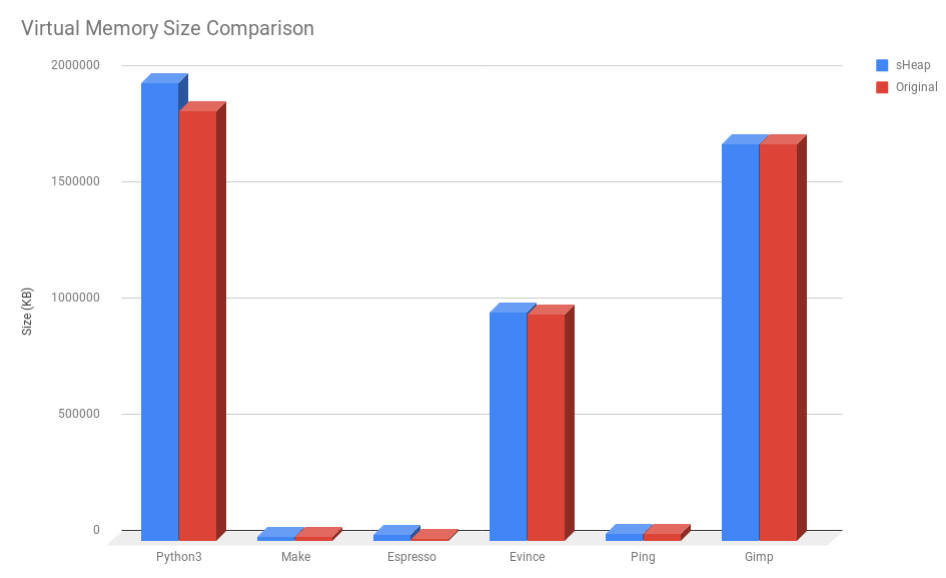
\includegraphics[width=\linewidth]{sheap-vsize-overhead-graph.png}
  \caption{sHeap Virtual Memory Overhead.}
  \label{fig:sheap-vsize-graph}
\end{figure}

sHeap has relatively minimal overhead in the VSize measurement for Gimp, evince, ping, 
and even Python 3. Espresso and Make have more of a discrepancy in this area, and the 
normalized results will be seen at the end of this subsection. RSS is a slightly similar 
story, as again both Make and Espresso appear worse, but to a greater intensity this time.

\begin{figure}[htbp]
  \centering
  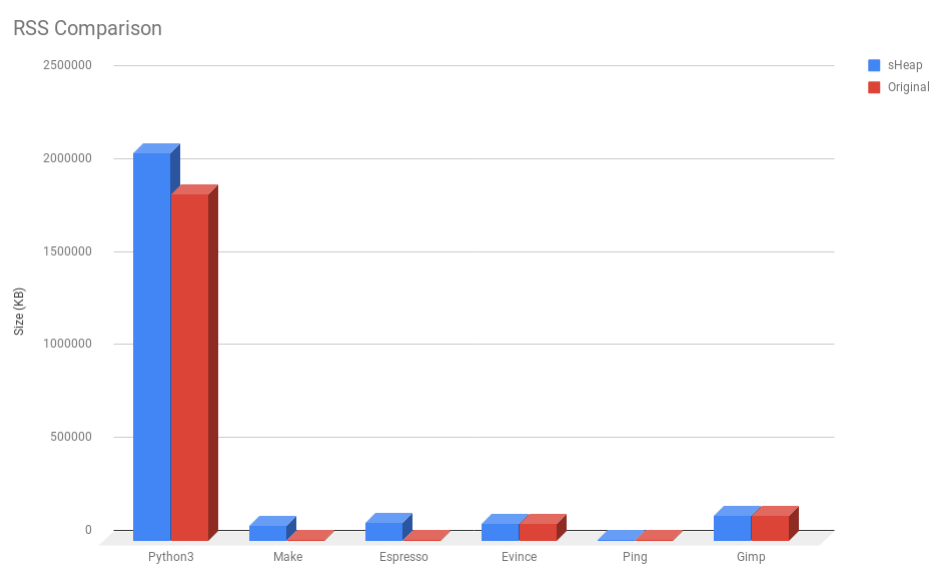
\includegraphics[width=\linewidth]{sheap-rss-overhead-graph.png}
  \caption{sHeap Resident Set Size Memory Overhead.}
  \label{fig:sheap-rss-graph}
\end{figure}

The other four programs all appear to be in a similar range of overhead for RSS. If we now look at 
\ref{fig:sheap-rss-graph}, we can see how much memory overhead is being incurred with sHeap now. 

\begin{figure}[htbp]
  \centering
  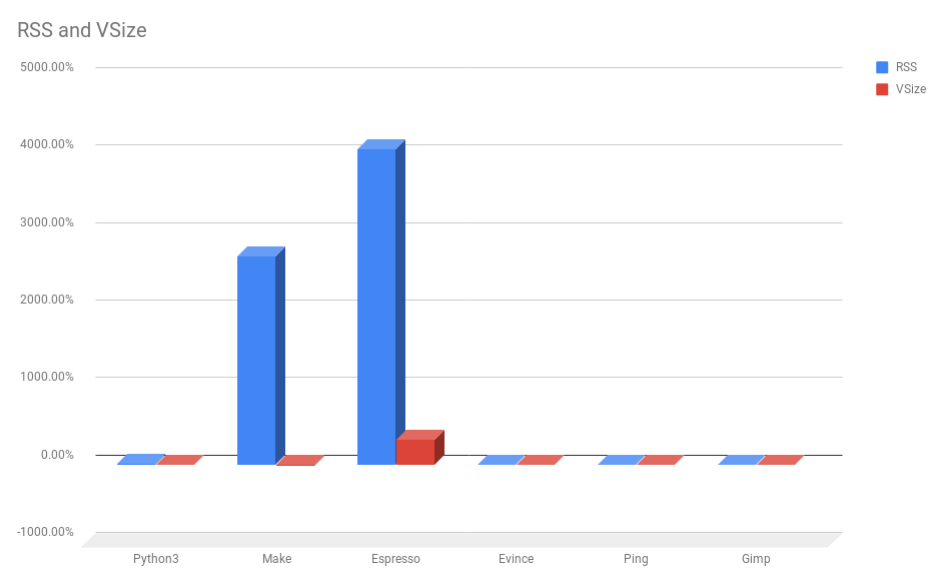
\includegraphics[width=\linewidth]{sheap-mem-overhead-graph.png}
  \caption{sHeap Memory Overhead.}
  \label{fig:sheap-mem-overhead-graph}
\end{figure}

Both Make and Espresso have significant RSS overhead, 2,691\% and 4,069\% respectively. Python 3 
however sits more comfortably at around 12\% RSS, while the remaining three programs are all 
under 1\%. With respect to VSize, Espresso is the only poorly performing benchmark coming in at 324\%.

\subsection{Runtime Overhead}
Now we turn out attention to the run-time overhead that is brought upon by the usage of sHeap. 
There are only four programs at work here as described in the section 5 introduction. Again, 
there are just two metrics that were tracked in the runtime department: User time and System 
time. If we look at the raw user time performance between sHeap and non-sHeap executions, we 
see sHeap performing worse across the board. This is especially true in the case of Make and 
Espresso, and less so in the case of Python 3 and ping. Ping logically makes sense as it is 
primarily bound by the I/O delays inherent to the nature of ping. System time is much worse 
in the case of Espresso and Make, where Espresso resulted in 4,913.33\% and Make yielded 
515.79\%. This is most likely  due to the lack of optimization for smaller allocations which 
forces a significantly higher rate of system calls to occur. Ping has a 100\% increase in system time due to the fact that 
it makes a single malloc call, and sHeap has to make one on initialization of its metadata which is doubling 
the number of allocation calls to the kernel. 

\begin{figure}[htbp]
  \centering
  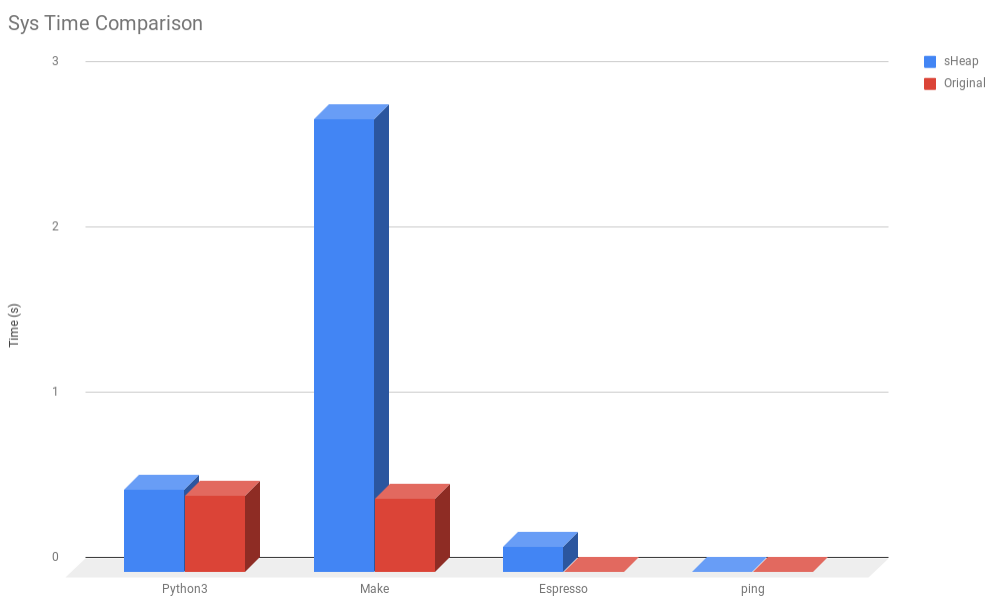
\includegraphics[width=\linewidth]{sheap-sys-time-overhead-graph.png}
  \caption{sHeap System Time Overhead.}
  \label{fig:sheap-sys-time-overhead-graph}
\end{figure}

\begin{figure}[htbp]
  \centering
  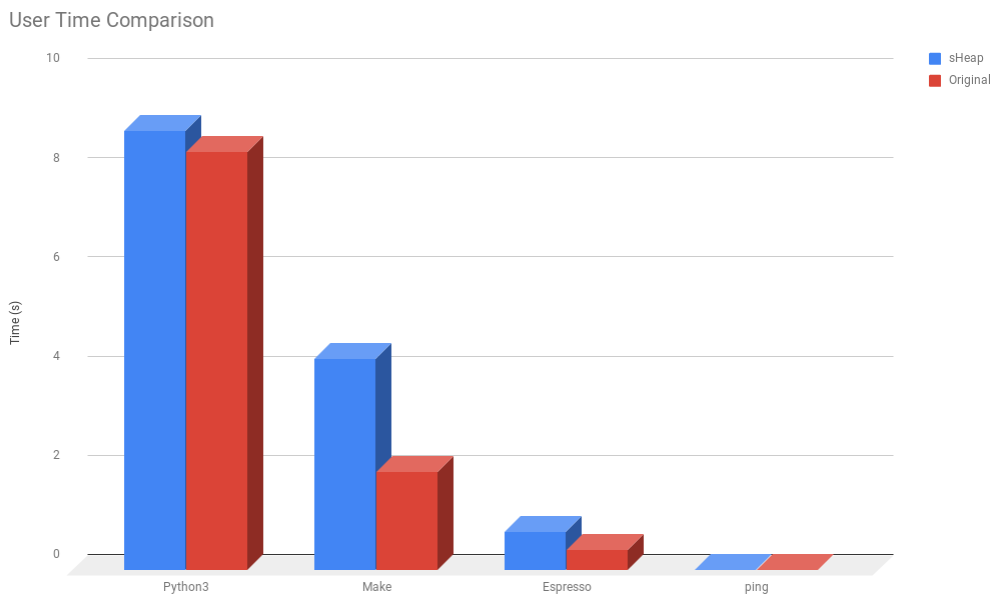
\includegraphics[width=\linewidth]{sheap-usr-time-overhead-graph.png}
  \caption{sHeap User Time Overhead.}
  \label{fig:sheap-user-time-overhead-graph}
\end{figure}

\subsection{Performance Hurdles}
The team understands where sHeap is having its performance hindered most severely. Due to 
the time constraint on the project, we had to choose which features/capabilities to tackle 
and give priority. In a perfect world, small allocations ($<16KB$) are performed in a more 
optimal manner. For example, the allocation of a small 16-byte structs should all be tucked 
together into a single virtual memory block, but as it stands now, a new block is allocated 
for each small allocation. This means both a syscall for each small allocation as well as 
the wasted virtual memory from only using 16 bytes from a whole 16KB block. Implementing a 
more efficient solution to smaller allocations would greatly increase performance from both 
the time and memory overhead points of view. Another side effect of this that relates 
primarily to time benchmarking is the lack of quality caching. Because allocations (especially 
small ones) are isolated into their own memory blocks, the principle of locality that drives 
the benefits of using a cache is all but useless. Fragmentation with sHeap is high, which means 
caches aren’t able to effectively perform their task.

\section{Limitations and Issues}
Our implementation introduces a number of limitations in order to ensure its functionality, as 
well as due to its prototype state. The most obvious limitation is that our heap manager 
relies on virtual memory being contiguous, and as a such all programs which use it cannot call 
sbrk in between malloc calls. This is because any such calls to sbrk will disturb the order, 
so the free list nodes don'’t match up with the appropriate allocated block. Programs that do use 
sbrk are detected however, and will cause the program to exit. Additionally, this system is 
also only applicable to 64 bit systems, due to the inefficiency of memory consumption, as well 
as due to the hash algorithm that was used in our pool hash table which expects 64 bit addresses. As mentioned in section 5-c, 
the implementation of improved handling for allocations less than 16KB is a big problem from a 
performance standpoint. This should be addressed in the future to make sHeap more usable. 
Another limitation is that sHeap requires a single large upfront allocation to store the 
out-of-band metaheap information and structures. This introduces a problem because now there is 
a restriction on how big the metaheap can grow (because of the continuity of memory issue from 
earlier). Further, in order to improve the performance of malloc calls, wrappers are only 
detected on subsequent calls, so the initial wrapper call is not detected as unusual, and as 
such it will cause the first one to have an allocation site in the wrapper. Further, we also 
can only detect the presence of a single layer of wrappers, and multiple layered wrappers are 
ignored - this is primarily due to the fact that we consider it exceptionally unusual to use 
multiple layers of malloc wrappers.

\section{Conclusion}
Dangling pointers represent a significant vulnerability space for attacks in the modern age. 
In this paper we have presented sHeap, a memory allocator designed to safely reuse heap space 
in order to prevent an attacker from being able to align heap objects in order to arbitrarily 
execute code through the use of dangling pointer exploits. It is able to do this by reliably 
identifying objects accurately based off of their allocation site, in a manner that is thread 
safe.

\begin{thebibliography}{00}
\bibitem{b1} Akritidis, P. ``Cling: A Memory Allocator to Mitigate Dangling Pointers,'' \textit{19th Usenix Security Symposium}, Washington DC, 2010. [Online]. Available: https://www.usenix.org/legacy/event/sec10/tech/full\_papers/Akritidis.pdf.
\bibitem{b2} Berger, E., and Zorn, B. ``DieHard: Probabilistic Memory Safety for Unsafe Languages,'' \textit{Proceedings of the ACM SIGPLAN Conference on Programming Language Design and Implementation}, ACM, NY, 2006, pp. 158--168. [Online]. Available: https://people.cs.umass.edu/~emery/pubs/fp014-berger.pdf.
\bibitem{b3} Lvin, V., Novark, G., Berger, E., and Zorn, B. ``Archipelago: Trading Address Space for Reliability and Security,'' \textit{SIGOPS Oper. Syst.}, Rev. 42, 2008, pp. 115--124. [Online]. Available: https://people.cs.umass.edu/~emery/pubs/asplos147-lvin.pdf.
\bibitem{b4} galengold, Espresso Logic Minimizer, 2017, GitHub Repository: https://github.com/galengold/espresso-logic.
\bibitem{b5} jeetsukumaran, Srupy: System Resource Usage Profiler, 2008, GitHub Repository: https://github.com/jeetsukumaran/Syrupy.
\end{thebibliography}

\end{document}
